\documentclass[journal]{IEEEtran}
\IEEEoverridecommandlockouts

\usepackage{amsmath,amssymb,amsfonts}
\usepackage{graphicx}
\usepackage{booktabs}
\usepackage{url}
\usepackage{xcolor}

% \todo{} marks something the author must confirm before submission. Set
% \todoson to 0 to hide them for a clean read.
\newcommand{\todo}[1]{\textcolor{red}{\textbf{[TODO: #1]}}}

\DeclareMathOperator{\rank}{rank}
\DeclareMathOperator*{\argmin}{arg\,min}
\newcommand{\bG}{\mathbf{G}}
\newcommand{\bS}{\mathbf{S}}
\newcommand{\bB}{\mathbf{B}}
\newcommand{\bW}{\mathbf{W}}
\newcommand{\bZ}{\mathbf{Z}}
\newcommand{\bY}{\mathbf{Y}}
\newcommand{\bg}{\mathbf{g}}
\newcommand{\CN}{\mathcal{CN}}
\newcommand{\Hank}{\mathcal{H}}
\newcommand{\reff}{r_{\mathrm{eff}}}
\newcommand{\dhs}{\Delta_{\mathrm{HS}}}

\begin{document}

\title{Effective-Rank Scaling of Hankel-Structured Channel\\
Estimation for Rydberg Atomic Quantum Receivers}

\author{Abdullah~Haatim%
\thanks{A.~Haatim is with the \todo{CONFIRM DEPARTMENT: taken from an earlier
draft in this project, not from a definitive source} Department of Electrical
and Electronics Engineering, Birla Institute of Technology and Science,
Pilani~--- Pilani Campus, India (e-mail:
f20220519@pilani.bits-pilani.ac.in).}}

\maketitle

\begin{abstract}
Rydberg atomic receivers measure field magnitude only, making multi-user
channel estimation a biased phase-retrieval problem. Imposing a low-rank
Hankel prior on the array response is known to help, but no published account
says when it helps and by how much, so the prior is applied wherever a sparse
multipath channel is assumed. We show that a single dimensionless quantity
governs the outcome: the effective rank of the per-user Hankel embedding
relative to its structural capacity. We derive that capacity, give an
oracle-free rank rule based on a held-out pilot residual, and show that the
number of users cancels from the associated compression ratio. Measured across
a fourfold range of array sizes, the ratio at which the prior ceases to pay is
invariant to within $0.07$, although the gain magnitude is not. Used
predictively, the relation forecast the gain on two channel models it was
never fitted to, one of them to within $0.13$~dB. The study is simulation
only, and the reference curve we report is genie-aided rather than a bound.
\end{abstract}

\begin{IEEEkeywords}
Rydberg atomic receiver, channel estimation, phase retrieval, Hankel matrix,
effective rank, structured low-rank approximation.
\end{IEEEkeywords}

\section{Introduction}

\IEEEPARstart{A}{tomic} receivers based on Rydberg states detect radio fields
through an optical readout whose output is proportional to field
\emph{magnitude}, discarding phase~\cite{cui2025,fancher2021}. Multi-user
channel estimation on such an array is therefore a phase-retrieval problem
with a known additive reference, and alternating-projection estimators of the
Gerchberg--Saxton family are the natural starting
point~\cite{gerchberg1972,netrapalli2015}. Recent work unrolls such an
estimator into a trained network~\cite{xiao2026}.

A separate and older idea is to exploit the geometry of the array response. If
each user's channel is a sum of a few plane waves on a uniform linear array
(ULA), its Hankel embedding is low rank, and projecting onto that set inside
the estimator loop suppresses noise that the unstructured iteration cannot
distinguish from signal~\cite{cadzow1988}. This works, and it is
straightforward to demonstrate on a sparse channel.

The difficulty is knowing when it applies. A practitioner asked to decide
whether the Hankel prior is worth its cost on a new deployment has, in the
current literature, only the qualitative advice that the channel should be
``sparse''. That advice is unusable, because the quantity that actually
matters is not the path count. A channel with sixteen paths on a
$32$-element array is algebraically full rank and yet has an effective rank of
$8.73$; its Hankel embedding is compressible even though nothing about it is
sparse.

\textbf{Contribution.} We replace the sparsity heuristic with a measurable
ratio and test it out of model.
\begin{enumerate}
\item We derive the structural capacity $\mathrm{cap}(N)=\lfloor N/2 \rfloor$
of the per-user Hankel embedding, and show that the number of users $K$
cancels from the compression ratio, predicting that the structural gain is
invariant in $K$.
\item We give an adaptive-rank estimator that selects the projection rank from
a held-out pilot residual, using no knowledge of the true path count.
\item We show that the ratio $\reff/\mathrm{cap}$ locates the \emph{boundary}
of the useful region to within $0.07$ across $N\in\{16,32,64\}$, while
stating plainly that the gain \emph{magnitude} does not collapse onto the same
axis, and quantifying the residual.
\item We use the relation predictively on two channel models it was never
fitted to, registering each prediction before measuring it.
\end{enumerate}

\textbf{Relation to rank projection in unrolled solvers.} Projecting onto a
low-rank set inside an iterative estimator is not new, and a rank projection
placed within projected gradient descent has been proposed for this
setting~\cite{xu_pgd}~\todo{VERIFY CITATION --- this work could not be located
or read; the distinction below is stated structurally and makes no claim about
its contents}. The distinction that matters is \emph{which} matrix is
constrained. Constraining the rank of the $N\times K$ channel matrix limits the
number of distinct spatial signatures across users, and is informative when
$K$ is large. The constraint used here is applied per user, to the Hankel
embedding of a single column, and encodes the harmonic structure of the ULA
manifold; it is informative even at $K=1$. The two are not substitutes, and
Sec.~\ref{sec:method} shows the second carries a $K$-invariance the first
cannot.

\section{System Model and Problem Formulation}
\label{sec:model}

An $N$-element ULA serves $K$ single-antenna users over $P$ pilot symbols.
Writing $\bG\in\mathbb{C}^{N\times K}$ for the channel, $\bS\in\mathbb{C}^{K
\times P}$ for the pilots and $\bB\in\mathbb{C}^{N\times P}$ for the known
reference beam, the receiver observes only magnitudes,
\begin{equation}
\bZ = \left| \bG\bS + \bB + \bW \right|,
\qquad \bW_{np}\sim\CN(0,\sigma^2),
\label{eq:fwd}
\end{equation}
with $|\cdot|$ elementwise. Estimating $\bG$ from $\bZ$ is phase retrieval
with a known bias term.

The $k$th user's channel follows a geometric model with $L_k$ paths,
\begin{equation}
\bg_k = \sum_{\ell=1}^{L_k}\alpha_{k\ell}\,
\mathbf{a}(\theta_{k\ell}),\qquad
[\mathbf{a}(\theta)]_n = e^{-j\pi n \sin\theta},
\label{eq:chan}
\end{equation}
so each column is a sum of complex exponentials in the element index.

\textbf{The reference curve is genie-aided.} Throughout, we plot an
unstructured least-squares estimate formed from the \emph{true} phase of the
noiseless field. It is not a bound. It presumes information no receiver has,
and it is restricted to unstructured least squares, so an estimator that
exploits channel structure may legitimately pass it; we observe exactly that
in a companion study. It is included only to indicate how much of the
magnitude-only penalty a given method removes.

\section{Proposed Method}
\label{sec:method}

\subsection{Hankel embedding and its capacity}

For $\bg\in\mathbb{C}^{N}$ and pencil parameter $p$, let $\Hank_p(\bg)$ be the
$(N-p)\times(p+1)$ Hankel matrix $[\Hank_p(\bg)]_{ij}=g_{i+j}$. Under
\eqref{eq:chan}, $\Hank_p(\bg_k)$ has rank $\min(L_k,N-p,p+1)$, so the largest
rank the embedding can express is
\begin{equation}
\mathrm{cap}(N)=\max_{p}\,\min(N-p,\,p+1)=\left\lfloor N/2 \right\rfloor ,
\label{eq:cap}
\end{equation}
attained at $p=\lfloor N/2\rfloor$. The two arguments cross between
$p=\lceil N/2\rceil-1$ and $p=\lceil N/2\rceil$; evaluating both gives
\eqref{eq:cap} for $N$ even and odd alike. A rank constraint at
$r=\mathrm{cap}(N)$ is satisfied by every vector and carries no information,
which fixes the scale against which any rank must be read.

\subsection{Why $K$ cancels}

Treated as unstructured, $\bG$ has $2NK$ real degrees of freedom. Under
\eqref{eq:chan} it is described by $3\sum_k L_k$ real parameters, two per
complex gain and one per angle. With $L_k\equiv\bar{L}$ the compression ratio
is
\begin{equation}
\frac{3\sum_k L_k}{2NK}=\frac{3K\bar{L}}{2NK}=\frac{3\bar{L}}{2N},
\label{eq:compress}
\end{equation}
% src: reports/trackD_normalization.md A1 (verified numerically for all
% (K, Lbar) in {2,3,4,6} x {3,5,7} to machine precision)
and $K$ cancels. Since the projection acts per user column, this predicts that
the structural gain is invariant in $K$ once pilot adequacy $P/2K$ is held
fixed --- a prediction we test in Sec.~\ref{sec:results}, and which the
per-user Hankel constraint makes but a constraint on $\rank(\bG)$ does not.

\subsection{Adaptive-rank HS-EM-GS}

The estimator alternates an expectation step over the unknown phases, a
Gerchberg--Saxton-type least-squares update, and a structural projection. For
a target rank $r$, let $\mathcal{P}_r(\bg)=\Hank_p^{\dagger}\!\left(
\Pi_r\!\left(\Hank_p(\bg)\right)\right)$, where $\Pi_r$ truncates to the $r$
leading singular values and $\Hank_p^{\dagger}$ averages along
antidiagonals. We note that a single application of $\mathcal{P}_r$ is not
idempotent: it is one step of an alternating projection between the rank set
and the Hankel set, not a projection onto their intersection.

The rank is not assumed. At each operating point we hold out a subset of
pilots, run the estimator for a reduced iteration count at every candidate
$r\in\{1,\dots,\mathrm{cap}(N)\}$, and select the $r$ minimising the residual
on the held-out pilots. The rule uses no ground truth. It also declines: when
it selects $r\ge \mathrm{cap}(N)$ the projection is the identity and the
estimator reduces to its unstructured counterpart, which is the behaviour we
observe on channels with no exploitable structure
(Sec.~\ref{sec:results}\,\ref{itm:oom}).

\subsection{The governing ratio}

For a channel column we measure the Roy--Vetterli effective
rank~\cite{royvetterli2007}~\todo{VERIFY CITATION} of its Hankel embedding,
$\reff=\exp(-\sum_i p_i \ln p_i)$ with $p_i=\sigma_i/\sum_j\sigma_j$, and
index results by $\reff/\mathrm{cap}(N)$. Effective rank, unlike $L$, is a
property of any channel rather than of one generator, and it is what makes the
out-of-model predictions in Sec.~\ref{sec:results} possible. It must be
computed on the noiseless channel: the effective rank of the \emph{estimate}
is set by the noise floor and collapses every configuration onto one value.

\section{Numerical Results}
\label{sec:results}

Table~\ref{tab:params} lists the configuration. Every cell draws SNR uniformly
and bins post hoc; the reported statistic is the paired per-trial median
within an SNR bin, with bootstrap 95\% confidence intervals. Pooled values are
reported where a single number per cell is needed and are dependent on the
uniform SNR design.

\begin{table}[!t]
\caption{Simulation parameters.}
\label{tab:params}
\centering
\small
\begin{tabular}{ll}
\toprule
Parameter & Value \\
\midrule
% src: trackD_urformer/config.py:120-129
Array elements $N$ & 32 (16, 64 in Sec.~\ref{sec:results}) \\
Users $K$ & 3 (2, 4 in the $K$ sweep) \\
Pilots $P$ & 20 (10, 15, 35 in the pilot sweep) \\
Paths per user $L_k$ & $\mathcal{U}\{3,7\}$ \\
Path gains $\alpha_{k\ell}$ & $\CN(0,1/L_k)$ \\
Angles $\theta_{k\ell}$ & $\mathcal{U}(-90^\circ,90^\circ)$ \\
SNR & $\mathcal{U}[-10,20]$~dB \\
Reference-to-signal ratio & 10~dB \\
Estimator iterations & 100 \\
% src: reports/trackD_partB9_analysis.json (per-cell "n")
Trials per cell & 83--874 (time-budgeted) \\
\bottomrule
\end{tabular}
\end{table}

\subsection{Gain across SNR at the default configuration}

Fig.~\ref{fig:snr} shows the improvement of adaptive-rank HS-EM-GS over
EM-GS. Every bin's confidence interval excludes zero, and the gain is flat in
SNR: it ranges over
% src: reports/trackD_partB9_analysis.json cells.B3_default.delta_hs.bins
$+2.374$ to $+3.108$~dB with no trend, pooling to $+2.680$~dB over
$n=274$ trials. The selected rank averages $4.59$, well below the
$\mathrm{cap}(32)=16$ ceiling and below the generator's own $L_{\max}=7$.
Against the genie-aided reference, the structural prior removes
% src: reports/trackD_partB9_analysis.json B4_oracle.B3_default
$58.2\%$ of the gap that EM-GS leaves.

\begin{figure}[!t]
\centering
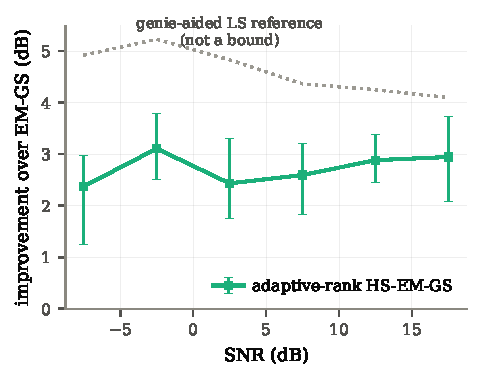
\includegraphics[width=\columnwidth]{fig/fig1_gain_vs_snr.pdf}
\caption{Improvement over EM-GS at the default configuration, paired per-trial
median with bootstrap 95\% CI. The genie-aided least-squares curve is
\emph{not} a bound; see Sec.~\ref{sec:model}.}
\label{fig:snr}
\end{figure}

\subsection{The boundary is invariant in $\reff/\mathrm{cap}$; the magnitude
is not}

Fig.~\ref{fig:boundary} places $N\in\{16,32,64\}$ on the $\reff/\mathrm{cap}$
axis. The value at which the gain crosses zero is
% src: reports/trackD_partB9_analysis.json B1_collapse.zero_crossing_*
$0.588$, $0.518$ and $0.544$ for $N=16$, $32$ and $64$ --- a spread of
$0.070$ across a fourfold change in aperture. The $N=16$ and $N=64$ crossings
are extrapolated from the last two measured points rather than bracketed by a
sign change, and should be read accordingly.

\textbf{The magnitude does not collapse, and we state the residual rather than
report a collapse.} Over the $\reff/\mathrm{cap}$ window both arrays cover,
$N=16$ lies above $N=64$ by
% src: reports/trackD_partB9_analysis.json B1_collapse.PRIMARY_internal_N16_vs_N64
a mean of $0.493$~dB and a maximum of $0.901$~dB, one-signed throughout and
monotone in $N$. We have no account of this residual. One candidate is the
coarseness of the pencil quantisation at small capacity --- $\mathrm{cap}(16)
=8$ admits eight distinct ranks against $32$ at $N=64$ --- but that is
untested, and the experiment that would settle it is a pencil sweep at fixed
$N$.

\begin{figure}[!t]
\centering
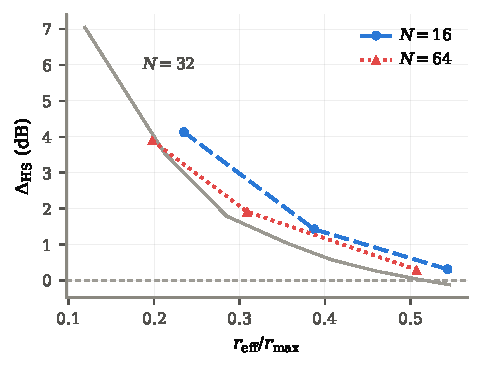
\includegraphics[width=\columnwidth]{fig/fig2_boundary_invariance.pdf}
\caption{$\dhs$ against $\reff/\mathrm{cap}$. The zero crossing is invariant
to within $0.070$ across $N\in\{16,32,64\}$; the gain \emph{magnitude} is not,
with $N=16$ exceeding $N=64$ by a one-signed mean of $0.493$~dB
(max.\ $0.901$~dB) at matched ratio. The $N=32$ curve is a reference measured
at a fixed 5~dB and is not paired with the other two.}
\label{fig:boundary}
\end{figure}

\subsection{Out-of-model prediction}
\label{itm:oom}

The relation is only useful if it transfers. We tested it on two channel
models it was never fitted to, computing $\reff/\mathrm{cap}$, reading a
predicted $\dhs$ off the relation, and \emph{committing the prediction to
version control before running the measurement}. The relation was not refitted
afterwards.

\textbf{Clustered Saleh--Valenzuela.} At $\reff/\mathrm{cap}=0.331$ the
relation predicts $+1.30$~dB. Measured:
% src: reports/trackD_partB9_analysis.json B6_xiao.B6_xiao_clustered
$+1.173$~dB, CI $[+1.017,+1.380]$, an error of $0.13$~dB with the prediction
inside the interval.

\textbf{A configuration with $L=10$ independent paths}~\cite{svconfig}~%
\todo{VERIFY CITATION --- the brief attributes this configuration to a
preprint that is not available here; the configuration is reproduced exactly
as specified but its attribution is unconfirmed}. At
% src: reports/trackD_step0_cui_prediction.json
$\reff/\mathrm{cap}=0.400$ the relation predicts $+0.648$~dB with interval
$[+0.367,+1.015]$ obtained by propagating the interquartile spread of $\reff$
through the same curve. Measured:
% src: reports/trackD_partB9_analysis.json B8_cui_measured
$+0.963$~dB, CI $[+0.808,+1.086]$ over $n=266$ trials. The measurement falls
inside the registered prediction interval and on the correct side of zero, but
the point estimate is $0.315$~dB low --- a larger error than on the clustered
model, and we report it as such rather than as a second $0.13$~dB hit. The two
tests together bound what the relation is good for: it places a previously
unseen channel on the correct part of the curve, and it is not accurate to a
tenth of a decibel in general.

\textbf{A partial match worth reporting.} On a second reading of the clustered
model in which all $40$ rays are drawn independently, $\reff/\mathrm{cap}$
rises to $0.748$ and the relation predicts a small \emph{negative} gain,
$-0.12$~dB. The measured median is
% src: reports/trackD_partB9_analysis.json B6_xiao.B6_xiao_literal
exactly $0.000$~dB. The magnitude is right to $0.12$~dB but \emph{the
mechanism is not what was predicted}: rather than degrading, the rank rule
declines to project at all in $29.1\%$ of trials, and the remaining trials
scatter symmetrically about zero. We report this as a partial match. It also
shows the rule discriminating without being told which channel it faces --- it
abstains in $29.1\%$ of trials on this model against $1.4\%$ on the clustered
one.

\begin{figure}[!t]
\centering
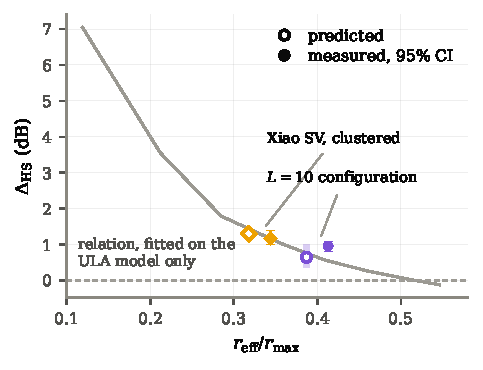
\includegraphics[width=\columnwidth]{fig/fig3_out_of_model.pdf}
\caption{Predictions registered before measurement, against measurement. The
relation is fitted on the ULA model of \eqref{eq:chan} only; neither channel
here was used to fit or tune it.}
\label{fig:oom}
\end{figure}

\subsection{Pilots, users, and cost}

\textbf{Pilots.} As the pilot count falls the structural gain grows
monotonically, from
% src: reports/trackD_partB9_analysis.json B7_P15_classical
$+2.300$~dB at $P=35$ to $+3.572$~dB at $P=10$, with disjoint confidence
intervals at the ends (Fig.~\ref{fig:pilots}); the change from $P=20$ to
$P=10$ is $+0.805$~dB at SNR $\ge 5$~dB. The selected rank falls with the
pilot count, $4.99\to4.29$, so the rule truncates harder exactly when the data
support less structure.

\textbf{Users.} The $K$-invariance predicted by \eqref{eq:compress} holds at
SNR $\ge 5$~dB, where $\dhs$ across $K\in\{2,3,4\}$ at fixed $P/2K$ spans
% src: reports/trackD_partB9_analysis.json B2_K_invariance
$0.095$~dB. Pooled over all SNR it does not: the spread is $0.294$~dB and
monotone in $K$. Our pre-registered falsifier was a monotone trend exceeding
$0.3$~dB, which this misses by $0.006$~dB, and we do not present that as a
pass. The pooled trend is driven by the bins below $0$~dB, where each cell
contributes roughly $45$ trials.

\textbf{Cost.} Per trial, single-threaded, relative to EM-GS:
% src: reports/trackD_cost_table.json
Gerchberg--Saxton $0.33\times$, fixed-rank HS-EM-GS $2.27\times$, and
adaptive-rank HS-EM-GS $10.40\times$. The rank search is the dominant cost;
where an operating point is stable, a rank selected once and reused recovers
most of the benefit at $2.27\times$.

\begin{figure}[!t]
\centering
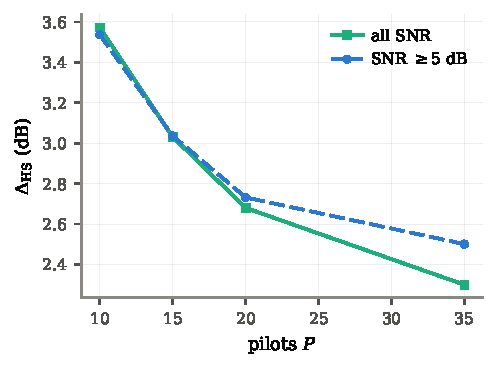
\includegraphics[width=\columnwidth]{fig/fig4_pilots.pdf}
\caption{The structural gain grows as pilots become scarce. Adaptive rank, at
the default configuration.}
\label{fig:pilots}
\end{figure}

\section{Conclusion}

The effective rank of the per-user Hankel embedding, taken relative to the
embedding's capacity $\lfloor N/2\rfloor$, determines whether an explicit
low-rank prior is worth applying. The ratio locates the boundary of the useful
region to within $0.070$ across a fourfold range of array sizes, and it
predicted the gain on two channel models it was never fitted to --- one to
within $0.13$~dB, the other inside a registered interval but $0.32$~dB off in
point estimate. Paired with an oracle-free rank rule that abstains when no
structure is present, this turns a qualitative sparsity heuristic into a
quantity a practitioner can compute before committing to the prior.

\textbf{Limitations.} These results are simulation only, with no measured
hardware or recorded channel data. They cover the geometric ULA model of
\eqref{eq:chan} and the two Saleh--Valenzuela configurations of
Sec.~\ref{sec:results}, and we make no claim beyond those channel families;
the gain magnitude in particular does not collapse onto the proposed axis, and
its residual is unexplained. Finally, we establish no fundamental bound: the
reference curve used throughout is genie-aided, presuming phase no receiver
observes, and is not a limit on achievable performance.

\bibliographystyle{IEEEtran}
\bibliography{refs}

\end{document}
